\documentclass[11pt, oneside]{article}   	% use "amsart" instead of "article" for AMSLaTeX format
\usepackage{geometry}                		% See geometry.pdf to learn the layout options. There are lots.
\geometry{letterpaper}                   		% ... or a4paper or a5paper or ... 
%\geometry{landscape}                		% Activate for rotated page geometry
%\usepackage[parfill]{parskip}    		% Activate to begin paragraphs with an empty line rather than an indent
\usepackage{graphicx}				% Use pdf, png, jpg, or eps§ with pdflatex; use eps in DVI mode
								% TeX will automatically convert eps --> pdf in pdflatex		
\usepackage{amssymb}
\usepackage{amsmath}
\usepackage{braket}
%SetFonts

%SetFonts


\title{Note on Error Mitigation}
\author{Takahiro Yamamoto}
%\date{}							% Activate to display a given date or no date

\begin{document}
\maketitle
\section{Type of error}
Qubit operations are susceptible to various types of errors due to imperfect control pulses, qubit-qubit couplings (crosstalk), and environmental noise. In order to improve qubit performance, it is necessary to identify the types and magnitudes of these errors and reduce them.
\begin{enumerate}
\item State preparation and measurement (SPAM)
\begin{enumerate}
\item intrinsic
\item extrinsic
\end{enumerate}
\item Gate infidelity
\begin{enumerate}
\item {1 qubit operation}
\item {2 qubit operation}
\end{enumerate}
\end{enumerate}

It will be useful to classify SPAM errors into two different types, which we will call {\em intrinsic} and {\em extrinsic}. 
Intrinsic SPAM errors are those that are inherent in the state preparation and measurement process. 
One example is an error initializing the $\ket{0}$ state due to thermal populations of excited states. 
Another is dark counts when attempting to measure, say, the $\ket{1}$ state. 
Extrinsic SPAM errors are those due to errors in the gates used to transform the initial state to the starting state (or set of states) for the experiment to be performed. 

Intrinsic SPAM errors are of particular relevance to fault-tolerant quantum computing, since it turns out that quantum error correction (QEC) requirements are much more stringent on gates than on SPAM. 

\begin{enumerate}
\item Dephasing
\item Amplitude and phasing damping
\item Homogeneous depolarizing
\end{enumerate}

\begin{enumerate}
\item Localized Markovian
\item Unbiased statistical fluctuation
\end{enumerate}

Below are some concrete examples of quantum noise and quantum operations. 
They are also important in understanding the practical effects of noise on quantum systems, and how noise can be controlled by techniques such as error-correction.

Quantum operations can be represented in the operator-sum representation:
\begin{equation}
\mathcal{E} (\rho) = \sum_k E_k \rho E^{\dagger}_k, 
\end{equation}
where the operators \{$E_k$\} are known as operation elements.

\subsection{Depolarizing}
Imagine we take a single qubit, and with probability $p$ that qubit is depolarized. 
That is, it is replaced by the completely mixed state, $I /2$. With probability $1-p$ the qubit is left untouched. 
The state of the quantum system after this noise is:
\begin{equation}
\mathcal{E} (\rho) = \frac{p I}{2} + (1-p) \rho
%\sqrt{p} I, \sqrt{1-p} Z
\end{equation}
In the operator-sum representation, 
\begin{equation}
\mathcal{E} (\rho) =\left({1 - \frac{3p}{4}} \right) \rho + \frac{p}{4} (X \rho X + Y \rho Y + Z \rho X)
%\sqrt{1 - \frac{3p}{4}} I
\end{equation}

\subsection{Amplitude damping}
the description of energy dissipation-effects due to loss of energy from a quantum system.
\begin{equation}
\mathcal{E} (\rho) = E_0 \rho E^{\dagger}_0 + E_1 \rho E^{\dagger}_1
\end{equation}
where 
\begin{equation}
E_0 = 
\begin{bmatrix}
1 & 0 \\
0 & \sqrt{1 - \gamma}
\end{bmatrix}, 
\end{equation}
\begin{equation}
E_1 = 
\begin{bmatrix}
0 & \sqrt{\gamma} \\
0 & 0
\end{bmatrix}.
\end{equation}
$\gamma$ can be thought of as the probability of losing energy.
The $E_1$ operation changes a $\ket{1}$ state into a $\ket{0}$ state, corresponding to the physical process of losing a quantum of energy to the environment. 
$E_0$ leaves $\ket{0}$ unchanged, but reduces the amplitude of a $\ket{1}$ state; 
physically, this happens because a quantum of energy was not lost to the environment, and thus the environment now perceives it to be more likely that the system is in the $\ket{0}$  state, rather than the $\ket{1}$ state.

$\mathcal{E}_{\textrm{GAD}}$, called generalized amplitude damping, is defined for single qubits by the operation elements
\begin{equation}
E_0 = \sqrt{p}
\begin{bmatrix}
1 & 0 \\
0 & \sqrt{1 - \gamma}
\end{bmatrix}, 
\end{equation}
\begin{equation}
E_1 = \sqrt{p}
\begin{bmatrix}
0 & \sqrt{\gamma} \\
0 & 0
\end{bmatrix},
\end{equation}
\begin{equation}
E_2 = \sqrt{1-p}
\begin{bmatrix}
\sqrt{1 - \gamma} & 0 \\
0 & 1
\end{bmatrix},
\end{equation}
\begin{equation}
E_3 = \sqrt{1-p}
\begin{bmatrix}
0 &0 \\
\sqrt{\gamma} & 0
\end{bmatrix}.
\end{equation}
where the stationary state $\rho_{\infty}$, which statisfies $\mathcal{E}_{\textrm{GAD}} (\rho_{\infty}) = \rho_{\infty}$ is,
\begin{equation}
\rho_{\infty} = 
\begin{bmatrix}
p &0 \\
0 & 1-p
\end{bmatrix}.
\end{equation}
When $\gamma$ is replaced with a time-varying function like $1-e^{t/T_1}$, you can visualize the effects of amplitude damping as a flow on the Bloch sphere, which moves every point in the unit ball towards a fixed point at $\ket{0}$.

\subsection{Phase damping}
A noise process that is uniquely quantum mechanical, which describes the loss of quantum information without loss of energy, is phase damping. 
The energy eigenstates of a quantum system do not change as a function of time, but do accumulate a phase which is proportional to the eigenvalue. 
When a system evolves for an amount of time which is not precisely known, partial information about this quantum phase -- the relative phases between the energy eigenstates -- is lost.
A phase kick, the angle of rotation $\theta$ is random. 
The randomness could originate, for example, from a deterministic interaction with an environment, which never again interacts with the system and thus is implicitly measured.
Let us assume that the phase kick angle $\theta$ is well represented as a random variable which has a Gaussian distribution 
$e^{- \theta^2/4 \lambda}$ 
with mean 0 and variance $2 \lambda$.

The random phase kicking causes the expected value of the off-diagonal elements of the density matrix to decay exponentially to zero with time, $e^{- \lambda}$. 
That is a characteristic result of phase damping.

\begin{equation}
\mathcal{E} (\rho) = E_0 \rho E^{\dagger}_0 + E_1 \rho E^{\dagger}_1
\end{equation}
where 
\begin{equation}
E_0 = 
\begin{bmatrix}
1 & 0 \\
0 & \sqrt{1 - \gamma}
\end{bmatrix}, 
\end{equation}
\begin{equation}
E_1 = 
\begin{bmatrix}
0 & 0 \\
0 & \sqrt{\gamma}
\end{bmatrix}.
\end{equation}

By applying the unitary freedom of quantum operations, we find that a unitary recombination of $E_0$ and $E_1$ gives a new set of operation elements for phase damping;
\begin{equation}
E^{\prime}_0 = \sqrt{\alpha} I
\end{equation}
\begin{equation}
E^{\prime}_1 = \sqrt{1-\alpha} Z,
\end{equation}
where $\alpha = (1 + \sqrt{1-\lambda})/2$.
Thus the phase damping quantum operation is exactly the same as the phase flip channel.

Phase damping is often referred to as a $T_2$ relaxation process, for historical reasons, where dephasing time is related to $\gamma$ as $e^{-t / 2T_2} = \sqrt{1 - \gamma}$. 
As a function of time, the amount of damping increases, corresponding to an inwards flow towards $\sigma_z$-axis.

\subsection{Phase flip}
\begin{equation}
\mathcal{E} (\rho) = p \rho + (1-p) Z \rho Z 
%\sqrt{p} I, \sqrt{1-p} Z
\end{equation}

\subsection{Bit flip}
The bit flip channel flips the state of a qubit from $\ket{0}$ to $\ket{1}$ (and vice versa) with probability $1-p$. 
It has operation elements

\begin{equation}
\mathcal{E} (\rho) = \sqrt{p} I \rho  \sqrt{p} I + \sqrt{1-p} X  \rho \sqrt{1-p} X 
%\sqrt{p} I, \sqrt{1-p} X
\end{equation}

\subsection{Bit-phase flip}
\begin{equation}
\mathcal{E} (\rho) = \sqrt{p} I \rho  \sqrt{p} I + \sqrt{1-p} X  \rho \sqrt{1-p} Y
%\sqrt{p} I, \sqrt{1-p} Y
\end{equation}

\section{Error models}
The most general form of a single-qubit unitary:
\begin{equation}
U (\theta, \phi, \lambda) = 
\begin{bmatrix}
\cos (\theta/2) & - e^{i \lambda} \sin (\theta/2) \\
e^{i \phi} \sin (\theta/2) & e^{i (\lambda + \phi)} \cos (\theta/2)
\end{bmatrix}, 
\end{equation}
It is implemented using three frame changes and two $X_{\pi/2}$ pulses. 

\begin{equation}
U_1(\lambda) = U (0, 0, \lambda) = 
\begin{bmatrix}
1 & 0 \\
0 & e^{i \lambda}
\end{bmatrix}, 
\end{equation}

\begin{equation}
U_2 (\phi, \lambda) = U (\pi/2, \phi, \lambda) = \frac{1}{\sqrt{2}}
\begin{bmatrix}
1 & - e^{i \lambda} \\
e^{i \phi} & e^{i (\lambda + \phi)}
\end{bmatrix}, 
\end{equation}
 In the IBM Q Experience, this is implemented by a pre- and post-frame change and a $X_{\pi/2}$ pulse
%https://quantumexperience.ng.bluemix.net/proxy/tutorial/full-user-guide/002-The_Weird_and_Wonderful_World_of_the_Qubit/004-advanced_qubit_gates.html

\subsection{Coherence}
The decay time,  ($T_1$) and dephasing time,  ($T_2$) 
\begin{equation}
f(t) = A e^{- t/T_1} + C
\end{equation}
for unknown parameters $A$, $C$, and $T_1$. 
If there are no SPAM errors,  $A = 1$ and $C = 0$.
Similarly, for $T_2$ and $T^*_2$,  the ground state population is expected to behave like
\begin{equation}
f(t) = A e^{- t/T^*_2} \cos( 2\pi f t + \phi ) + C
\end{equation}
respectively; both with $A = C = 1/2$ in the lack of SPAM errors.

\subsection{Hamiltonian Characterization}
Measuring $ZZ$
perform an experiment to measure $ZZ$ between a pair of qubits. 
$ZZ$ here is defined as the energy shift on the $\ket{11}$ state,
\begin{equation}
H = \frac{\omega_0}{2} (1 - \sigma_{Z, 0}) + \frac{\omega_1}{2} (1 - \sigma_{Z, 1}) + \xi \ket{11} \bra{11}
%f(t) = A e^{- t/T^*_2} \cos( 2\pi f t + \phi ) + C
\end{equation}
The experiment to measure $\xi$ is to perform a Ramsey experiment on Q0 (H-t-H) and repeat the Ramsey with Q1 in the excited state. 
The difference in frequency between these experiments is the rate $\xi$. 
ZZ rates are typically $\approx$100kHz so we want Ramsey oscillations around 1MHz.
12 numbers ranging from 10 to 1000, logarithmically spaced
%https://github.com/Qiskit/qiskit-tutorials/blob/master/qiskit/ignis/hamiltonian_and_gate_characterization.ipynb

\subsection{Amplitude Error Characterization for Single Qubit Gates}
Measure the amplitude error in the single qubit gates. 
Here this measures the error in the $\pi/2$ pulse. 
Note that we can run multiple amplitude calibrations in parallel. 
% Here we measure on qubits 2 and 4.
This shows the sequence of the calibration, which is repeated application of $Y_{\pi} = e^{i (\pi/2) Y} = U_2(0, 0)$. 
Note that the measurements are mapped to a minimal number of classical registers in order of the qubit list.

Suppose error model where each $Y_{\pi}$ gate has error
\begin{equation}
\begin{bmatrix}
\cos (\theta) & - \sin (\theta) \\
\sin (\theta) & \cos (\theta)
\end{bmatrix}.
\end{equation}
Excited state population can be fit as:
\begin{equation}
C - \frac{1}{2} \cos \left[ \left( \theta + \frac{\pi}{2} \right) (x + 1) \right]
\end{equation}
where $x$ is the number of gate repetitions and $\theta$ is the error for the pulse (amplitude/error). [TODO: fill the gap]

\subsection{Angle Error Characterization for Single Qubit Gates}
Measure the angle between the $X$ and $Y$ gates

Gate sequence for measuring the angle error
$U_2(0, 0) U_1 (2 \theta) U_2(- \pi/2, \pi/2) U_2(- \pi/2, \pi/2) \cdots$

where the $U_1$ gates are added errors to test the procedure

\subsection{Amplitude Error Characterization for CNOT Gates}
This looks for a rotation error in the CNOT gate, ie., if the gate is actually $CR_X(\pi/2+\delta)$ measure $\delta$. 
This is very similar to the single qubit amplitude error calibration except we need to specify a control qubit (which is set to be in state $\ket{1}$) and the rotation is a $\pi$.

Suppose error model where each CNOT gate has error
\begin{equation}
\begin{bmatrix}
I & O \\
O & e^{i \theta X}
\end{bmatrix}.
\end{equation}

\begin{equation}
C + \frac{1}{2} \sin \left[ \left( \theta + \pi\right) x \right]
\end{equation}
where $x$ is the number of gate repetitions and $\theta$ is the amplitude error for the pulse.
See: [https://qiskit.org/documentation/ignis/characterization.html]

\subsection{Angle Error Characterization for CX Gates}
Measure the angle error $\theta$ in the CNOT gate, i.e., $CR_{\cos(\theta)X+\sin(\theta)Y}(\pi/2)$ with respect to the angle of the single qubit gates.

\subsection{Measurement Error and Mitigation}
% https://github.com/Qiskit/qiskit-tutorials/blob/master/community/ignis/measurement_error_mitigation.ipynb
The last step of a typical quantum experiment is to perform a measurement on the qubits in the circuit. 
Although the qubit state $\ket{\psi}$ (or more generally the density matrix $\rho$) is the general description of the quantum state, in a typical strong projective measurement our measurement projects the general state into a specific computational state $\ket{x}$ (where $x$ is a bitstring, e.g.,  1001010) The probability of measuring bitstring $x$ is given by: 
\begin{equation}
P_x = \mathrm{Tr}(\bra{x} \rho \ket{x})
\end{equation}
Therefore, the measurement process is stochastic. 
The above distribution of $x$ given a state $\rho$ is true only in the absence of measurement errors. 
There are multiple sources of possible measurement error, all of which are dependent on the physical mechanism of measurement in the system. 
For superconducting qubits coupled to readout cavities [1,2,3,4,5] the state of the qubit is determined by measurement the response of a microwave tone incident on the readout cavity. The cavity signal is measured for some time where $V(t)$ is the complex amplitude of the signal which is converted to a single complex number based on a measurement kernel 
\begin{equation}
V = \int_0^{T} V(t) K(t) dt
\end{equation}
which is then turned into a bit by a nonlinear discriminator [6]. 
The simplest example being if $|V| < V_0$ then the qubit was in state 0 and otherwise the qubit was in state 1.

As discussed in [6] there are classical sources of noise on the signal that lead to misidentification of the qubit state, but it can also happen that the qubit decays due to $T_1$ during the measurement. There are other sources of crosstalk (to numerous to enumerate) such as classical crosstalk on the lines and crosstalk between resonantors on chip. All of these issues lead to a new probability distribution $\tilde{P}_{\rho}$ for a given state. Given certain assumptions about these errors and appropriate calibration we can attempt to correct the skew in the probability distribution on average.

References
[1] Alexandre Blais, Ren-Shou Huang, Andreas Wallraff, S. M. Girvin, and R. J. Schoelkopf, Cavity quantum electrodynamics for superconducting electrical circuits: An architecture for quantum computation, https://arxiv.org/abs/cond-mat/0402216

[2] Jay Gambetta, Alexandre Blais, D. I. Schuster, A. Wallraff, L. Frunzio, J. Majer, M. H. Devoret, S. M. Girvin, and R. J. Schoelkopf. Qubit-photon interactions in a cavity: Measurement induced dephasing and number splitting https://arxiv.org/abs/cond-mat/0602322

[3] Alexandre Blais, Jay Gambetta, A. Wallraff, D. I. Schuster, S. M. Girvin, M. H. Devoret, and R. J. Schoelkopf. Quantum information processing with circuit quantum electrodynamics. https://arxiv.org/abs/cond-mat/0612038

[4] Jay Gambetta, W. A. Braff, A. Wallraff, S. M. Girvin, R. J. Schoelkopf. Protocols for optimal readout of qubits using a continuous quantum nondemolition measurement. https://arxiv.org/abs/cond-mat/0701078

[5] Jay Gambetta, Alexandre Blais, M. Boissonneault, A. A. Houck, D. I. Schuster and S. M. Girvin. Quantum trajectory approach to circuit QED: Quantum jumps and the Zeno effect. https://arxiv.org/abs/0709.4264

[6] Colm A. Ryan, Blake R. Johnson, Jay M. Gambetta, Jerry M. Chow, Marcus P. da Silva, Oliver E. Dial and Thomas A. Ohki. Tomography via Correlation of Noisy Measurement Records. https://arxiv.org/abs/1310.6448

\subsection{Constructing a Full Calibration Matrix}
The assumption of the error mitigation technique is that we can prepare each of the basis states with very low error. Given this assumption, in separate experiments we can prepare one of the $2^n$ states and then measure the outputs in all $2^n$ states. Normalizing these outputs and making each set of output probabilities for a given prepared state the columns of a matrix we obtain the matrix $\mathbf{A}$ which translates the ideal probability distribution of the state $\rho$ ($P_\rho$) into the experimental probability distribution $\tilde{P}_{\rho}$ 
\begin{equation}
\tilde{P}_{\rho} = \mathbf{A} \cdot P_{\rho}
\end{equation}

\subsection{Error models}
\begin{equation}
\Lambda(\rho) = \sum_k E_k \rho E^{\dagger}_k
\end{equation}

\begin{align}
E_1 &= \frac{1 + \sqrt{1 - \gamma - \lambda}}{2} I + \frac{1 - \sqrt{1 - \gamma - \lambda}}{2} Z \\
E_2 &= \frac{\sqrt{\gamma}}{2} (X + iY) \\
E_1 &= \frac{\sqrt{\lambda}}{2} (I - Z)
\end{align}

\begin{equation}
\Lambda(\rho) 
\to \sum_{A \in \mathcal{A}} A^{\dagger} \Lambda(A \rho A^{\dagger}) A
= \sum_{A \in \mathcal{A}} p_A A^{\dagger} \rho A
\end{equation}

\begin{equation}
\mathcal{A} = \{ I, X, Y, Z \}
\end{equation}

\section{Qubit characterization methods}
Several methods of qubit characterization are currently available\footnote{Introduction to Quantum Gate Set Tomography, D.~Greenbaum, arXiv:1509.02921}. 
In chronological order of their development, the main techniques are:
\begin{enumerate}
\item quantum state tomography (QST)
\item quantum process tomography (QPT)
\item randomized benchmarking (RB)
\item quantum gate set tomography (GST)
\end{enumerate}

\subsection{Quantum state tomography (QST)}

\subsection{Quantum process tomography (QPT)}
A quantum operation on a $d$-dimensional quantum system can be completely determined by experimentally measuring the output density matrices produced from $d^2$ pure state inputs.

\subsection{Randomized benchmarking (RB)}

\subsection{Quantum Volume}
Quantum Volume (QV) is a single-number metric that can be measured using a concrete protocol on near-term quantum computers of modest size. 
The QV method quantifies the largest random circuit of equal width and depth that the computer successfully implements. 
Quantum computing systems with high-fidelity operations, high connectivity, large calibrated gate sets, and circuit rewriting toolchains are expected to have higher quantum volumes.

The Quantum Volume Protocol
A QV protocol (see [1]) consists of the following steps:

\subsubsection{Step 1: Generate QV sequences}
It is well-known that quantum algorithms can be expressed as polynomial-sized quantum circuits built from two-qubit unitary gates. 
Therefore, a model circuit consists of $d$ layers of random permutations of the qubit labels, followed by random two-qubit gates (from $SU(4)$). 
When the circuit width $m$ is odd, one of the qubits is idle in each layer.

More precisely, a QV circuit with depth $d$ and width $m$, is a sequence $U = U^{(d)} \cdots U^{(2)}U^{(1)}$ of $d$ layers: 
\begin{equation}
U^{(t)} = U^{(t)}_{\pi_t(m'-1),\pi_t(m)} \otimes \cdots \otimes U^{(t)}_{\pi_t(1),\pi_t(2)}
\end{equation}
 each labeled by times $t = 1 ... d$ and acting on $m' = 2 \lfloor n/2 \rfloor$ qubits. Each layer is specified by choosing a uniformly random permutation $\pi_t \in \mathcal{S}_m$ of the $m$ qubit indices and sampling each $U^{(t)}_{a,b}$, acting on qubits $a$ and $b$, from the Haar measure on $SU(4)$.

% In the following example we have 6 qubits Q0,Q1,Q3,Q5,Q7,Q10. We are going to look at subsets up to the full set (each volume circuit will be depth equal to the number of qubits in the subset)

\subsubsection{Step 2: Simulate the ideal QV circuits}
The quantum volume method requires that we know the ideal output for each circuit, so we use the statevector simulator in Aer to get the ideal result.

\subsubsection{Step 3: Calculate the heavy outputs}
To define when a model circuit $U$ has been successfully implemented in practice, we use the heavy output generation problem. The ideal output distribution is 
$p_U(x) = | \bra{x} U \ket{0} |^2$, where $x \in \{0,1\}^m$ is an observable bit-string.

Consider the set of output probabilities given by the range of $p_U(x)$ sorted in ascending order 
$p_0 \leq p_1 \leq \dots \leq p_{2^m-1}$. 
The median of the set of probabilities is  $p_{\mathrm{med}} = (p_{2^{m-1}} + p_{2^{m-1}-1})/2$, and the heavy outputs are 
\begin{equation}
H_U = \left\{ x \in \{0,1\}^m \mid p_U(x) > p_{\mathrm{med}} \right\}.
\end{equation}
 The heavy output generation problem is to produce a set of output strings such that more than two-thirds are heavy.
% As an illustration, we print the heavy outputs from various depths and their probabilities (for trial 0):

\subsubsection{Step 4: Define the noise model}
We define a noise model for the simulator. To simulate decay, we add depolarizing error probabilities to the CNOT and $U$ gates.

\subsubsection{Step 5: Calculate the average gate fidelity}
The average gate fidelity between the $m$-qubit ideal unitaries $U$ and the executed $U'$ is: 
\begin{equation}
F_{\mathrm{avg}}(U,U') = \frac{|\mathrm{Tr}(U^{\dagger}U')|^2/2^m+1}{2^m+1}
\end{equation}

The observed distribution for an implementation $U'$ of model circuit $U$ is $q_U(x)$, and the probability of sampling a heavy output is: $$ h_U = \sum_{x \in H_U} q_U(x)$$
%As an illustration, we print the heavy output counts from various depths (for trial 0):

\subsubsection{Step 6: Calculate the achievable depth}
The probability of observing a heavy output by implementing a randomly selected depth $d$ model circuit is: 
\begin{equation}
h_d = \int_U h_U dU
\end{equation}

The achievable depth $d(m)$ is the largest $d$ such that we are confident that $h_d > 2/3$. 
In other words, 
\begin{equation}
h_1, h_2,\cdots,h_{d(m)} > \frac{2}{3} \text{ and } h_{d(m+1)} \leq \frac{2}{3}
\end{equation}

We now convert the heavy outputs in the different trials and calculate the mean $h_d$ and the error for plotting the graph.

\subsubsection{Step 7: Calculate the Quantum Volume}
The quantum volume treats the width and depth of a model circuit with equal importance and measures the largest square-shaped (i.e., $m = d$) model circuit a quantum computer can implement successfully on average.

The quantum volume $V_Q$ is defined as 
\begin{equation}
\log_2 V_Q = \arg\max_{m} \min (m, d(m))
\end{equation}
We list the statistics for each depth. 
For each depth we list if the depth was successful or not and with what confidence interval. For a depth to be successful the confidence interval must be $> 97.5 \%$.

References
[1] Andrew W. Cross, Lev S. Bishop, Sarah Sheldon, Paul D. Nation, and Jay M. Gambetta, Validating quantum computers using randomized model circuits, https://arxiv.org/pdf/1811.12926
[2] S. Aaronson, L. Chen, Complexity-Theoretic Foundations of Quantum Supremacy Experiments, https://arxiv.org/pdf/1612.05903
[3] Quantum Supremacy and the Complexity of Random Circuit Sampling, https://arxiv.org/pdf/1803.04402

\subsection{Quantum gate set tomography (GST)}

GST arose from the observation that QPT is inaccurate in the presence of SPAM errors. 
In QPT, the starting states must form an informationally complete basis of the Hilbert-Schmidt space on which the gate being estimated acts. 
These are typically created by applying gates to a given initial state, usually the $\ket{0}$ state, and these gates themselves may be faulty.

According to recent results from IBM, a 50-fold increase in intrinsic SPAM error reduces the surface code threshold by only a factor of 3-4. 
Therefore QPT -- the accuracy of which degrades with increasing SPAM -- would not be able to determine if a qubit meets threshold requirements when the ratio of intrinsic SPAM to gate error is large.

This is not an issue for extrinsic SPAM errors, which go to zero as the errors on the gates go to zero. 
Nevertheless, extrinisic SPAM error interferes with diagnostics: as an example, QPT cannot distinguish an over-rotation error on a single gate from the same error on all gates. 
In addition, Merkel, et al. have found that, for a broad range of gate error -- including the thresholds of leading QEC code candidates -- the ratio of QPT estimation error to gate error increases as the gate error itself decreases. 
This makes QPT less reliable as gate quality improves.

Extrinsic SPAM error is also unsatisfactory from a theoretical point of view: QPT assumes the ability to perfectly prepare a complete set of states and measurements. 
In reality, these states and measurements are prepared using the same faulty gates that QPT attempts to characterize. 
One would like to have a characterization technique that takes account of SPAM gates self-consistently. 
We shall see that GST is able to resolve all of these issues.

Another approach to dealing with SPAM errors is provided by randomized benchmarking. 
RB is based on the idea of twirling -- the gate being characterized is averaged in a such a way that the resulting process is depolarizing with the same average fidelity as the original gate. 
The depolarizing parameter of the averaged process is measured experimentally, and the result is related back to the average fidelity of the original gate. 
This technique is independent of the particular starting state of the experiment, and therefore is not affected by SPAM errors. 
However, RB has several shortcomings which make it unsatisfactory as a sole characterization technique for fault-tolerant QIP. 
For one thing, it is limited to Clifford gates, and so cannot be used to characterize a universal gate set for quantum computing. 
For another, RB provides only a single metric of gate quality, the average fidelity. 
This can be insufficient for determining the correct qubit error model to use for evaluating compatibility with QEC. 
Several groups have shown that qualitatively different errors can produce the same average gate fidelity, and in the case of coherent errors the depolarizing channel inferred from the RB gate fidelity underestimates the effect of the error. 
Finally, RB assumes the errors on subsequent gates are independent. 
This assumption fails in the presence of non-Markovian, or time-dependent noise. 
GST suffers from this assumption as well, but the long sequences used in RB make this a more pressing issue.

Despite these apparent shortcomings, RB has been used with great success by several groups to measure gate fidelities and to diagnose and correct errors. 
RB also has the advantage of scalability -- the resources required to implement RB (number of experiments, processing time) scale polynomially with the number of qubits being characterized. 
QPT and GST, on the other hand, scale exponentially with the number of qubits. 
As a result, these techniques will foreseeably be limited to addressing no more than 2-3 qubits at a time. 

GST and RB may end up complementing each other as elements of a larger characterization protocol for any future multi-qubit quantum computer.

TODO: summarize them in table.
\begin{table}[h]
\begin{tabular}{l | l | l | l | l}
method & assumption & advantage & disadvantage & scalability \\
\hline
quantum state tomography &  &  &  &  \\
quantum process tomography &  &  &  &  \\
randomized benchmarking &  &  &  & \\
quantum gate set tomography &  &  &  & 
\end{tabular}
\end{table}

\section{Type of error mitigation technics}
There are four types of errors that can result in infidelity in the variational quantum simulation: 
\begin{enumerate}
\item errors due to limited generality of the trial wave function, which may only be able to describe the simulated system approximately; 
\item shot noise (TODO: definition) in measurments 
\item errors due to noise in the quantum machine, e.g., decoherence and quantum gate infidelity.
\end{enumerate}

Type of error mitigation technics are listed as:
\begin{enumerate}
\item Error extrapolation
\item Quasiprobability decomposition
\item Quantum subspace expansion. quantum channels
\item Process tomography protocols
\begin{enumerate}
\item Gate set tomography
\end{enumerate}
\end{enumerate}

\subsection{Homogeneous and inhomogeneous scaling}
%\subsubsection{Motivation}
\subsubsection{Theory}
Consider the case in which the effect of machine noise is to depolarize the ancillary qubit at a fixed level; \textit{i.e.}, the output of the quantum computer becomes 
$\left< X \right> = \eta \left< X \right>^{(0)}$, 
where $\eta$ is a constant independent of the quantum circuit. 
%In this case, all equation coefficients are scaled as 

An example of the homogeneous scaling is the case of balanced measurement errors. 
Errors in the measurement on the ancillary qubit (see Fig.?) can be modeled as follows: 
\begin{enumerate}
\item
If the state of the qubit is $\ket{0}$ the measurement outcome is correct with the probability $(1-p_0)$ and the outcome is incorrect with the probability $p_0$
\item
If the state of the qubit is $\ket{1}$ the measurement outcome is correct with the probability $(1-p_1)$ and the outcome is incorrect with the probability $p_1$
\end{enumerate}

\begin{figure}[t]
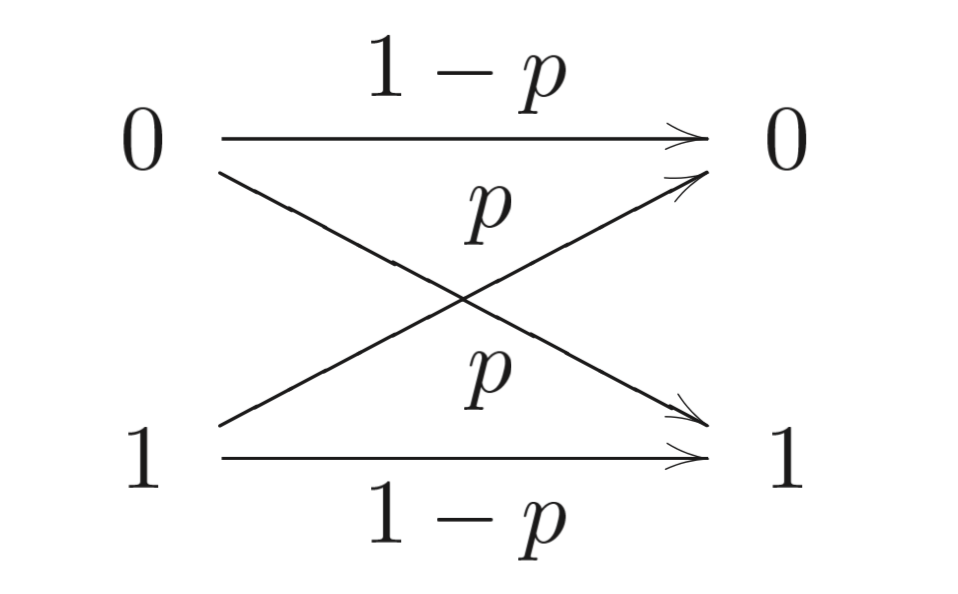
\includegraphics[width=8cm]{./img/bitflip}
\centering
\end{figure}

Then the expectation value is 
$\left< X \right> = (p_1 - p_0) + (1 - p_0 - p_1) \left< X \right>^{(0)}$, 

If measurement errors are balanced, \textit{i.e.}, $p_0 = p_1$, the effect of measurement errors is a fixed scaling factor 
$\eta = 1 - p_0 - p_1$, which does not result in computing errors. 
Therefore, the hybrid algorithm is inherently insensitive to measurement errors on the ancillary qubit if these errors are balanced. 
Note also that if single-qubit gates are reliable, one can flip the qubit before the measurement so that measurement errors are effectively balanced.
Measurement errors can be corrected even if they are not balanced. 
If $p_0$ and $p_1$ can be evaluated by benchmarking measurement operations, one can easily work out the true value 
$\left< X \right>^{(0)}$ using the value obtained from the real machine: 
$\left< X \right>^{(0)} = [\left< X \right> - (p_1 - p_0)]/(1 - p_0 - p_1)$
We note that when error probabilities are higher, the denominator is smaller, which means that we need to evaluate $[\left< X \right>$ with a higher accuracy in order to achieve the same accuracy of $\left< X \right>^{(0)}$\footnote{PhysRevX.7.021050}

\subsubsection{Experiment}
\subsubsection{Summary}

\subsection{Error extrapolation}
\subsubsection{Motivation}
\subsubsection{Theory}
Errors in an operation are stochastic if the operation is described by a superoperator $\mathcal{N} \mathcal{U}$ and $\mathcal{N}$ has the form 
$\mathcal{N} = (1 - \epsilon) \mathcal{I} + \mathcal{E}$. 
Here, $\mathcal{U}$ is the ideal operation without errors, $\mathcal{N}$ is the superoperator describing the effect of the noise, $\mathcal{I}$ is an identity operation, and errors $\mathcal{E}$ occur with the probability $\epsilon$. 
Here, $\mathcal{E}$ is a valid quantum operation, \textit{i.e.}, trace-preserving completely positive map.

Given an initial state $\rho$, after a sequence of operations, the final state of the quantum computer is
$\rho = \mathcal{N}_L \mathcal{U}_L \cdots \mathcal{N}_{\ell} \mathcal{U}_{\ell} \cdots \mathcal{N}_1 \mathcal{U}_1 \rho$

where $\mathcal{N}_{\ell} \mathcal{U}_{\ell}$ denotes the $\ell$-th operation. 
Taking into account the fact that errors are stochastic, the outcome can be rewritten in the form
\begin{equation}
\left< X \right> = \left(1 - r \sum \epsilon_{\ell} \right) \left< X \right>^{(0)} + r  \left< X \right>^{(1)} + \mathcal{O}(r^2),
\end{equation}
where $r$ is a convenient scale factor. 
For more detailed discussion see [PhysRevX.7.021050].
If probabilities of errors are tunable, we can infer the value of $\left< X \right>^{(0)}$ by measuring values of $\left< X \right>$ of a set of
different factors $r$ [see Fig.?]. 

To infer the value of $\left< X \right>^{(0)}$, first, we take $N_X$ values of $r$ and measure $\left< X \right>$ with $r_1, \cdots, r_X$ , where
we can take $r_1 = 1$. 
Then, we fit the output as $\left< X \right> (r) = \left< X \right>^{(0)} + \chi r$ and obtain the value of $\left< X \right>^{(0)}$.
In this way, the first-order contribution of machine noise can be corrected. 
Similarly, by considering second-order terms in the expansion Eq.?, we can fit data using a function with second-order terms.

Using the extrapolation, we can reduce the effect of the machine noise. 
However, the final estimation of $\left< X \right>^{(0)}$ may still be different from its actual value, and the error in the extrapolation depends on the shot noise in estimating each $\left< X \right> (r)$.

\begin{figure}[t]
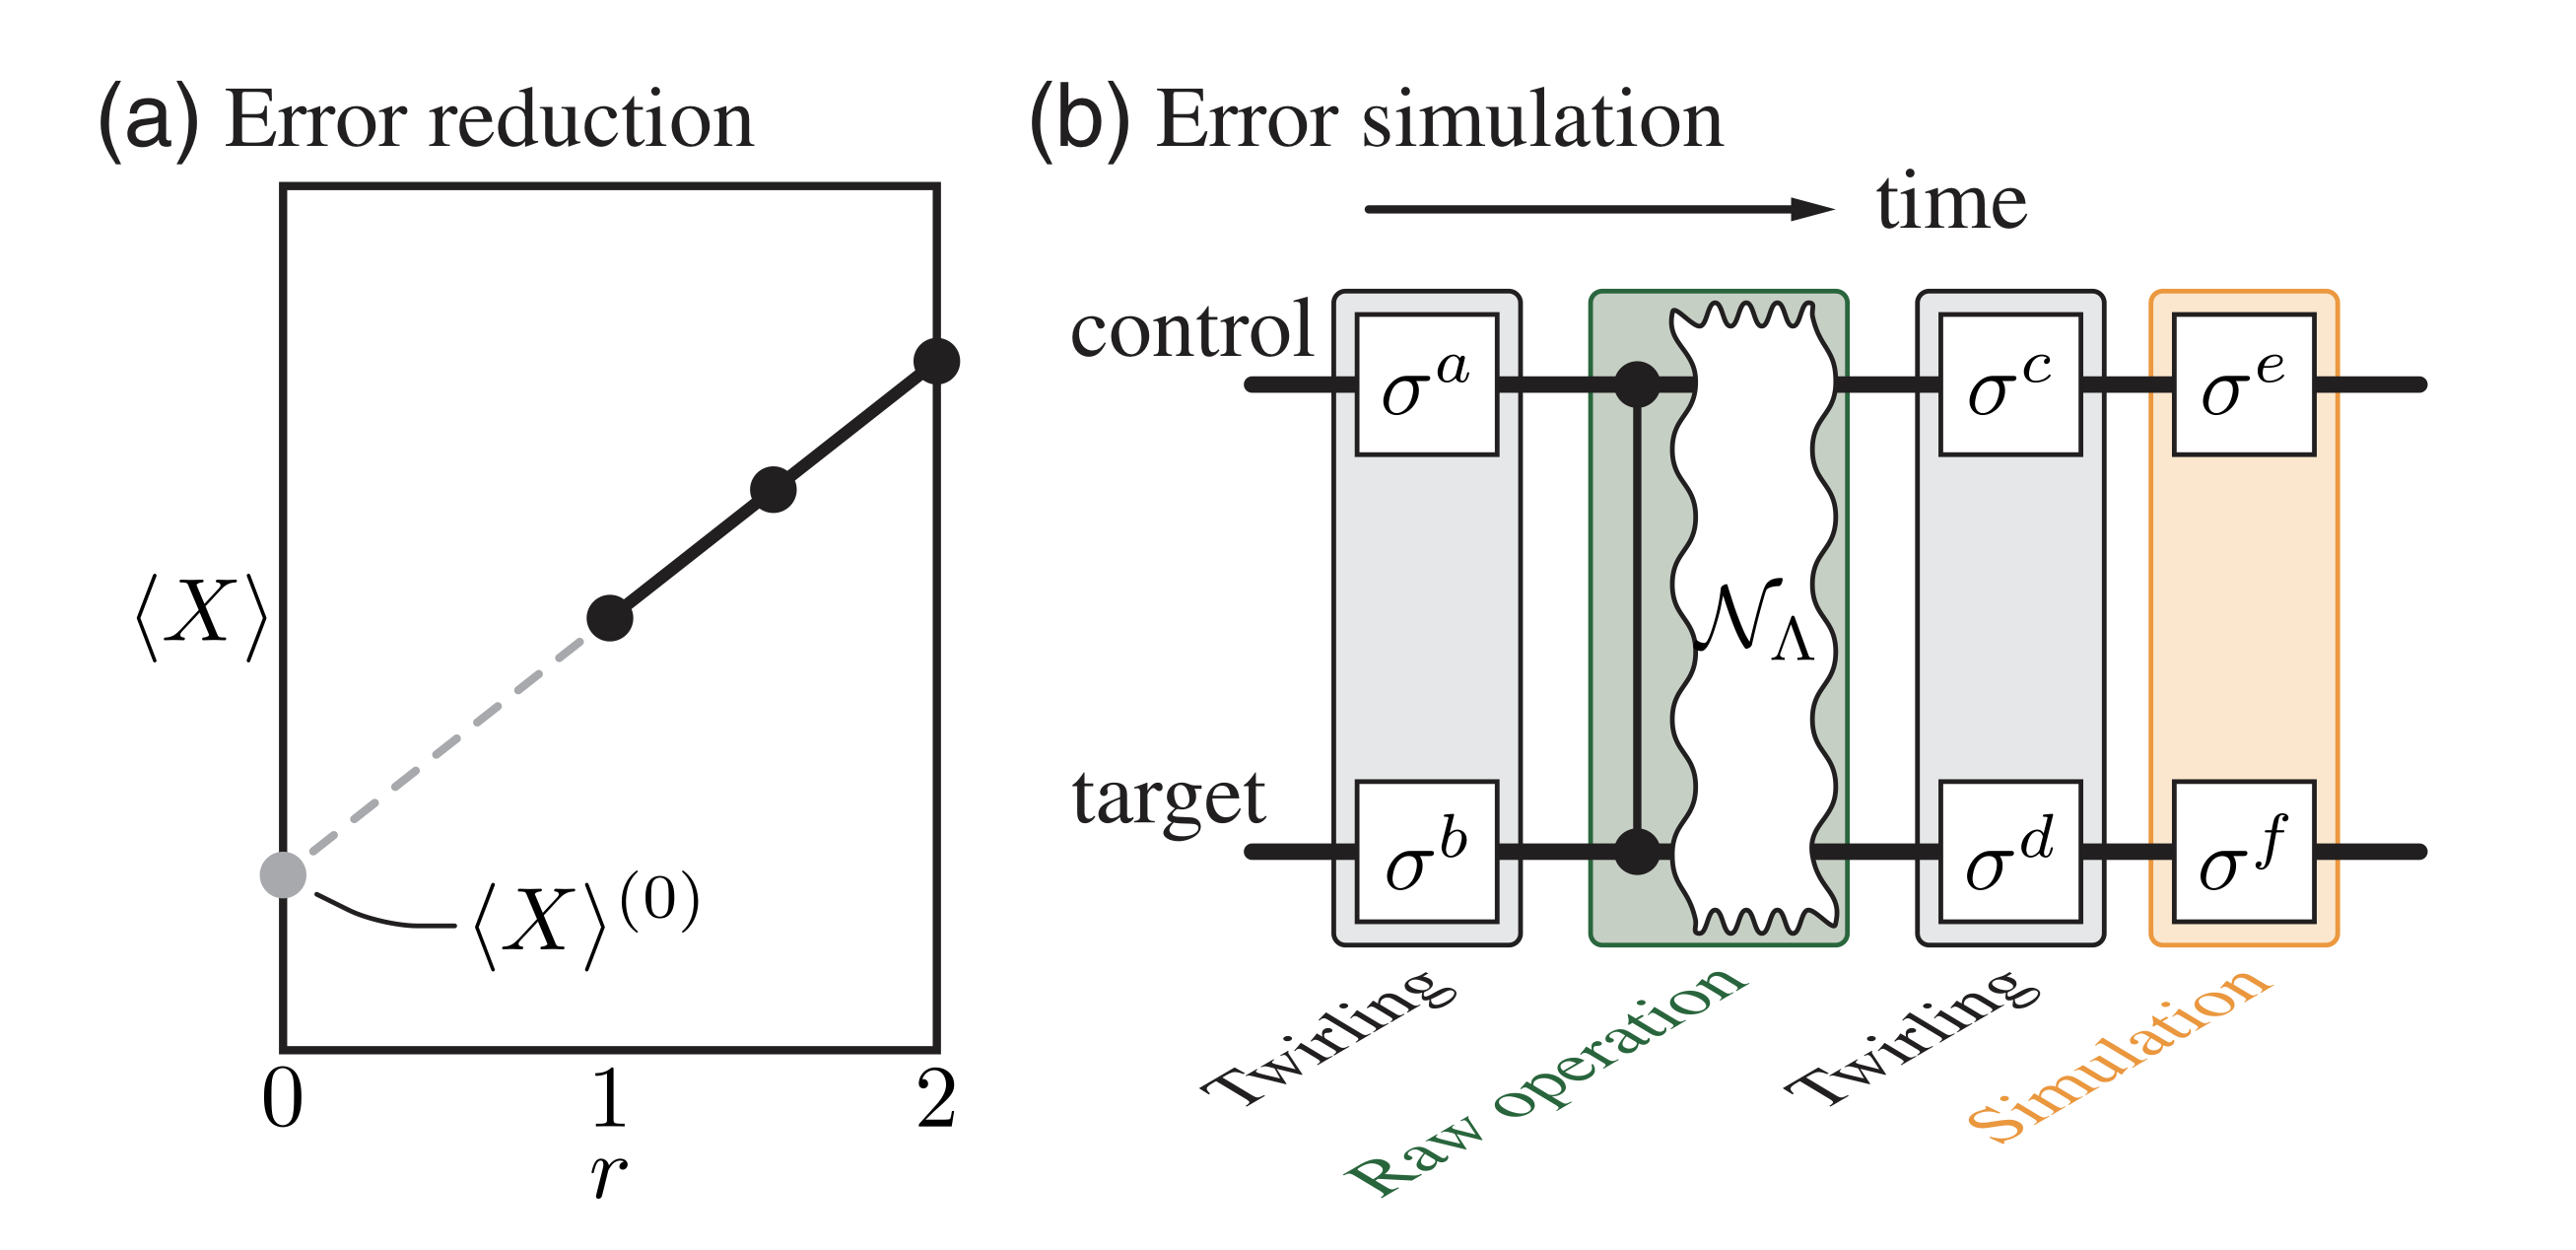
\includegraphics[width=8cm]{./img/PRX7_021050}
\centering
\end{figure}

The error-reduction protocol only works for small-size circuits, which are used in the hybrid algorithm, while the Trotterization algorithm usually needs large-size circuits. 
The true value $\left< X \right>^{(0)}$ can be inferred when the contribution of high-order terms is much smaller than the contribution of lower-order terms.

The total rate of errors in the circuit with $N_g$ gates is approximately $1 - (1 - \epsilon)^{N_g} = N_g \epsilon + (N_g \epsilon)^2 / 2 + \cdots$.

When there are too many gates in the circuit or the error rate is too high,$N_g \epsilon \gtrapprox 1$, the quantum state will be populated with errors, and one cannot retrieve the true value $\left< X \right>^{(0)}$ even if we consider high-order terms in the interpolation.

\subsubsection{Experiment}
\subsubsection{Summary}

\subsection{Error twirling}
TODO: fill in

\subsection{Quasiprobability decomposition}
\subsubsection{Motivation}
\subsubsection{Theory}
Utility of ``twirling'' operations in minimizing the cost\footnote{Error Mitigation for Short-Depth Quantum Circuits, K. Temme, S. Bravyi, and J. M. Gambetta, Phys. Rev. Lett. 119, 180509}.
For the extrapolation method, their optimisation is to observe that typically for the classes of noise most common in experiments it is appropriate to assume that the expected values of the observation will decay exponentially with he severity of the circuit noise, rather than polynomial.

\subsubsection{Experiment}
\subsubsection{Summary}

\subsection{Process tomography protocols}
Localized Markovian errors
\subsubsection{Motivation}
\subsubsection{Theory}
Single-qubit Clifford gates and measurements are universal in  computing expectation values.
Any quantum operation is a linear map.
Single qubit Clifford gates and measurements yield a complete set of linear independent maps.
Any error can be simulated or subtracted by decomposition of the error using complete operation set.

By combining GST and the complete set decomposition, any localized Markovian errors in the QC can be systematically mitigated, 
so that the error in the final computational output is due to unbiased statistical fluctuation.

\subsubsection{Experiment}
\subsubsection{Summary}

\section{Summary}
\begin{enumerate}
\item {Error mitigation method}
\item {Applicable error type}
\item {Efficiency}
\item {Cost (per qubit)}
\end{enumerate}

\appendix
\section{Topological QC}
Fault-tolerant quantum computing can be achieved by encoding qubits in non-Abelian anyons in topological materials\footnote{A. Kitaev, Fault-Tolerant Quantum Computation by Anyons, Ann. Phys. (Amsterdam) 303, 2 (2003).}

\section{Quantum error correction}
However, quantum error correction involves a substantial multiplication of resources; the number of physical qubits required may be orders of magnitude greater than the number of error-free logical qubits seen by the algorithm. A recent study audited the cost of implementing Shor’s algorithm to solve a classically infeasible task and found that, even with state-of-the-art techniques for magic-state distillation, the machine would need over six million of today’s highest- quality qubits\footnote{J. O’Gorman and E. T. Campbell, Quantum Computation with Realistic Magic State Factories, Phys. Rev. A 95, 032338 (2017)}.
% J. O’Gorman and E. T. Campbell, Quantum Computation with Realistic Magic State Factories, Phys. Rev. A 95, 032338 (2017)

\section{Dynamics simulation of  quantum system}
Dynamics must be studied when properties cannot be determined from static features. 
This has motivated dynamical versions of many well-known techniques, e.g., nonequilibrium dynamical mean-field theory\footnote{H. Aoki, N. Tsuji, M. Eckstein, M. Kollar, T. Oka, and P. Werner, Nonequilibrium Dynamical Mean-Field Theory and Its Applications, Rev. Mod. Phys. 86, 779 (2014).}, 
the time-dependent variational quantum Monte Carlo method\footnote{G. Carleo, F. Becca, M. Schiro, and M. Fabrizio, Localization and Glassy Dynamics of Many-Body Quantum Systems, Sci. Rep. 2, 243 (2012).}, 
time-dependent tensor network methods\footnote{A. J. Daley, C. Kollath, U. Schollwock, and G. Vidal,
Time-Dependent Density-Matrix Renormalization-Group Using Adaptive Effective Hilbert Spaces, J. Stat. Mech. (2004) P04005., M. C. Banuls, M. B. Hastings, F. Verstraete, and J. I. Cirac, Matrix Product States for Dynamical Simulation of Infinite Chains, Phys. Rev. Lett. 102, 240603 (2009).}, 
and, of course, time-dependent density functional theory\footnote{E. Runge and E. K. U. Gross, Density-Functional Theory for
Time-Dependent Systems, Phys. Rev. Lett. 52, 997 (1984).}. 

A new approach\footnote{Ying Li and Simon C. Benjamin, Efficient Variational Quantum Simulator Incorporating Active Error Minimization, Physical Review X 7, 021050 (2017)} is based on the variational method, and our hope is that it could be implemented using small- size quantum circuits, i.e., quantum circuits with a small number of quantum operations that suffer significant noise compared with fault-tolerant quantum computers.

Variational methods have numerous applications in the numerical study of many-body quantum systems: for example, 
density functional theory\footnote{R. O. Jones, Density Functional Theory: Its Origins, Rise to Prominence, and Future, Rev. Mod. Phys. 87, 897 (2015).}, 
the matrix product state method\footnote{D. Perez-Garcia, F. Verstraete, M. M. Wolf, and J. I. Cirac, Matrix Product State Representations, Quantum Inf. Comput. 7, 401 (2007).}, 
and simulating molecular dynamics using the variational principle\footnote{H. Feldmeier and J. Schnack, Molecular Dynamics for
Fermions, Rev. Mod. Phys. 72, 655 (2000).}

\end{document}  